%%%%%%%%%%%%%%%%%%%%%%%%%%%%%%%%%%%%%%%%%
% Journal Article
% LaTeX Template
% Version 1.3 (9/9/13)
%
% This template has been downloaded from:
% http://www.LaTeXTemplates.com
%
% Original author:
% Frits Wenneker (http://www.howtotex.com)
%
% License:
% CC BY-NC-SA 3.0 (http://creativecommons.org/licenses/by-nc-sa/3.0/)
%
%%%%%%%%%%%%%%%%%%%%%%%%%%%%%%%%%%%%%%%%%

%----------------------------------------------------------------------------------------
%	PACKAGES AND OTHER DOCUMENT CONFIGURATIONS
%----------------------------------------------------------------------------------------

\documentclass[twoside]{article}

\usepackage{lipsum} % Package to generate dummy text throughout this template

\usepackage[sc]{mathpazo} % Use the Palatino font
\usepackage[T1]{fontenc} % Use 8-bit encoding that has 256 glyphs
\linespread{1.05} % Line spacing - Palatino needs more space between lines
\usepackage{microtype} % Slightly tweak font spacing for aesthetics

\usepackage[hmarginratio=1:1,top=32mm,columnsep=20pt]{geometry} % Document margins
\usepackage{multicol} % Used for the two-column layout of the document
\usepackage[hang, small,labelfont=bf,up,textfont=it,up]{caption} % Custom captions under/above floats in tables or figures
\usepackage{booktabs} % Horizontal rules in tables
\usepackage{float} % Required for tables and figures in the multi-column environment - they need to be placed in specific locations with the [H] (e.g. \begin{table}[H])
\usepackage{hyperref} % For hyperlinks in the PDF
\usepackage{graphicx}
\usepackage{amsmath}
\usepackage{bbm}

\usepackage{lettrine} % The lettrine is the first enlarged letter at the beginning of the text
\usepackage{paralist} % Used for the compactitem environment which makes bullet points with less space between them

\usepackage{abstract} % Allows abstract customization
\renewcommand{\abstractnamefont}{\normalfont\bfseries} % Set the "Abstract" text to bold
\renewcommand{\abstracttextfont}{\normalfont\small\itshape} % Set the abstract itself to small italic text

\usepackage{titlesec} % Allows customization of titles
\renewcommand\thesection{\Roman{section}} % Roman numerals for the sections
\renewcommand\thesubsection{\Roman{subsection}} % Roman numerals for subsections
\titleformat{\section}[block]{\large\scshape\centering}{\thesection.}{1em}{} % Change the look of the section titles
\titleformat{\subsection}[block]{\large}{\thesubsection.}{1em}{} % Change the look of the section titles

\usepackage{fancyhdr} % Headers and footers
\pagestyle{fancy} % All pages have headers and footers
\fancyhead{} % Blank out the default header
\fancyfoot{} % Blank out the default footer
\fancyhead[C]{} % Custom header text
\fancyfoot[RO,LE]{\thepage} % Custom footer text

%----------------------------------------------------------------------------------------
%	TITLE SECTION
%----------------------------------------------------------------------------------------

\title{\vspace{-15mm}\fontsize{24pt}{10pt}\selectfont\textbf{Options Prices in the Fat Tail Domain}} % Article title

\author{
\large
\textsc{Christian Drappi}\\[0.5mm] % Your name
\normalsize \href{mailto:cld22@duke.edu}{netid: cld22} \\ \\ % Your email address
\normalsize Duke University \\ % Your institution
\normalsize Math 582: Financial Derivatives \\
\normalsize Professor Arlie Petters \\
\vspace{-5mm}
}
\date{}

%----------------------------------------------------------------------------------------

\begin{document}

\maketitle % Insert title

\thispagestyle{fancy} % All pages have headers and footers

%----------------------------------------------------------------------------------------
%	ABSTRACT
%----------------------------------------------------------------------------------------

\begin{abstract}

\noindent In 1973, Fischer Black and Myron Scholes published the groundbreaking paper titled "The Pricing of Options and Corporate Liabilities". This work, combined with Robert Merton's "Theory of Rational Option Pricing" of the same year provided a framework to approximate the correct price of a European option. Originally, the authors had assumed that the logarithmic returns of the underlying security followed a Gaussian distribution. Historical data falsifies this assumption. Since then, academics, quants and traderd have worked toward building a more accurate model of stock prices. This paper explores one such approach - the Variance Gamma process - both theoretically and computationally.

\end{abstract}

%----------------------------------------------------------------------------------------
%	ARTICLE CONTENTS
%----------------------------------------------------------------------------------------

\begin{multicols}{2} % Two-column layout throughout the main article text

\section{Introduction}

\lettrine[nindent=0em,lines=3]{A} ccording to popular legend, the Ancient Greek Thales of Miletus bought the world's first call option \cite{tibben2006real}. He predicted that the season's olive production would be abnormally high. Acting on this, he bought the right but not the obligation to use a fixed number of olive presses for the upcoming spring. When the olive harvest was indeed larger than expected, he exercised his right to rent the olive pressers from their owner, and then rented out the same presses at the market price during olive season. By locking in a low rental rate for himself but charging a higher price after demand spiked, Thales profited on his deal.

Since then, options have boomed in popularity; today, options trading is a multi-trillion dollar industry. Much of this growth can be attributed to the work of three academics: Black, Scholes and Merton. Their 1973 papers mathematically validated options markets as they derived a single, rational price of a European call option.

With their academic expertise in options pricing, Myron Scholes and Robert Merton joined the board of directors of Long-Term Capital Management, a newly founded hedge fund. While the firm performed outstandingly in the first three years, it collapsed after the 1997 Asian and 1998 Russian financial crises. Perhaps an incomplete understanding of risk caused this downturn. In his 2001 book \emph{When Genius Failed: The Rise and Fall of Long-Term Capital Management}, Roger Lowenstein summarized LTCM's trading strategies as "picking up nickels in front of a bulldozer" \cite{lowenstein2001genius}. The firm capitalized on small victories by selling many options that were essentially lottery tickets: when someone hit the jackpot, LTCM went under.

Some people, such as bestselling author Nassim Taleb, saw it coming. "Taleb predicted that hedge funds like Long Term Capital Management were headed for trouble, because they did not understand this notion of fat tails", wrote popular author Malcolm Gladwell \cite{gladwell}. Before writing his famous book \emph{The Black Swan}, Taleb spent his time trading options with the exact opposite strategy that drove Scholes and Merton's firm to the ground. The trader would take long positions on out-of-the-money calls and puts when he believed that the market underestimated the probability of moving into-the-money before expiration \cite{gladwell}. Because these options were underpriced, he could make many trades, win on a very small percentage of them and profit immensely. On his Twitter feed Taleb states, "I did 700,000 trades in career, was "wrong" on between 650,000 and 695,000. Wish I did more. Kapish?" \cite{twitter}.

As the game of options trading gets tougher, one must go beyond the original BSM model when pricing options. In \emph{Non-Gaussian Merton-Black-Scholes Theory}, Svetlana I. Boyarchenko and Sergei Z. Levendorskii write about one class of approaches that assume the underlying follows a regular Levy process of the exponential type, a class of non-Gaussian models for shocks \cite{ngmbs}. This paper will contrast original BSM results with the results that Boyarchenko and Levendorskii's theory produces.

%------------------------------------------------

\section{Shortcomings of Gaussian Options Pricing}
After analyzing years of market data, it has become clear that logarithmic returns of stocks usually do not follow a Gaussian distribution. The distribution of log returns looks similar to a Gaussian, except that a Gaussian distribution has thin tails (to be precise, every moment of the Gaussian is finite). The distribution of a stock's log returns, on the other hand, has fat tails.

\subsection{Deviations from Normality}

On "Black Monday", the Dow Jones Industrial Average fell by 25.6\% - a movement 22 standard deviations away from the mean \cite{22sigmas}. If we lived in the Gaussian world, the probability of making this move would be about $1.4 \times 10^{-107}$. To put this in perspective, the stock market could run every day from the beginning of the universe (about 5 trillion days), and the probability of a movement this extreme happening is almost zero: orders of magnitude less than one divided by the number of atoms in the universe ($10^{80}$).

Below, we plot the empirical, standardized logarithmic returns of the S\&P 500 index from January 2, 1957 to December 31, 2013 \cite{yahoofinance}. On the same figure, we plot the standard normal density. Clearly, the empirical distribution does not match the Gaussian as the peak is larger yet the tails are fatter \cite{Rlang} \cite{ggplot2}.

\begin{center}
	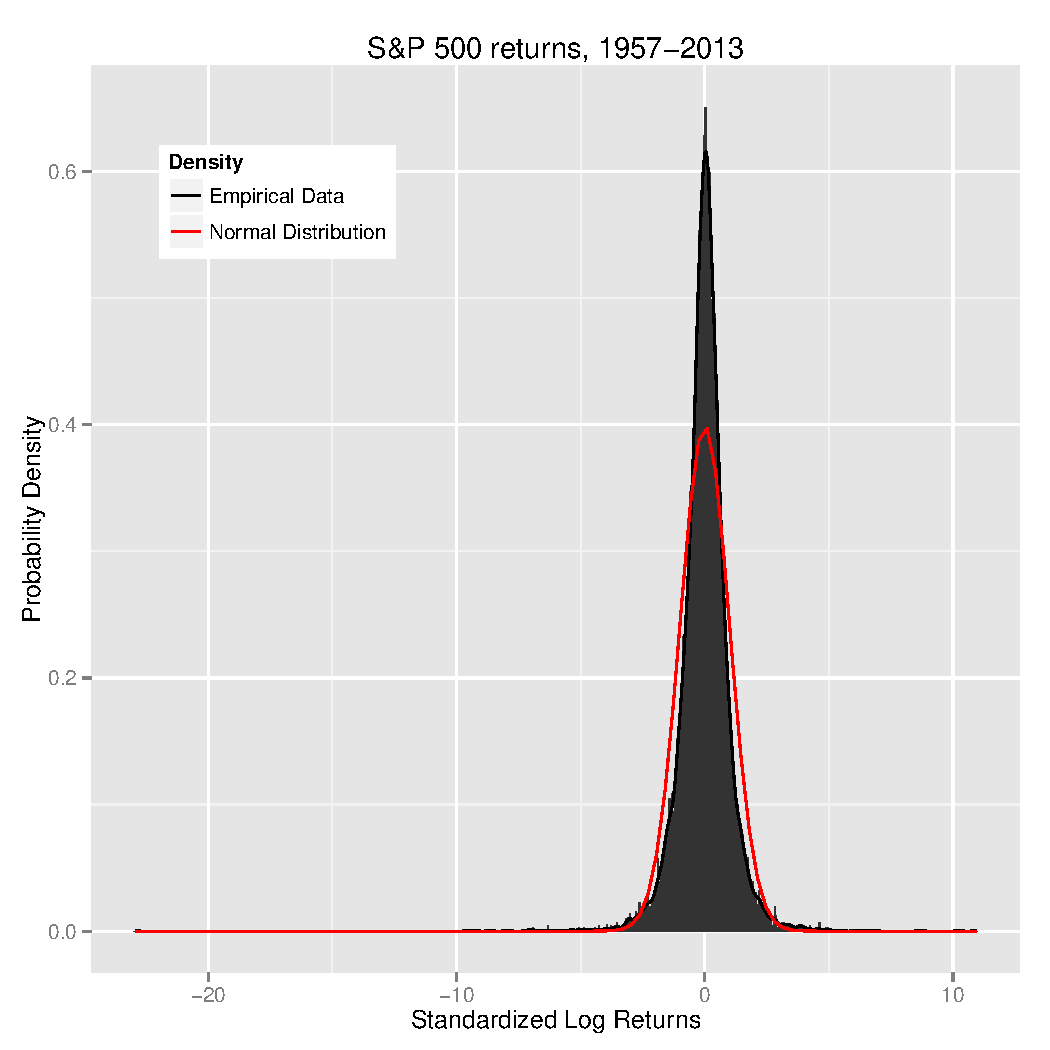
\includegraphics[width=0.44\textwidth]{SP500}
\end{center}

\subsection{Asymmetric Exposures}

When the distribution of a stock's returns has fat (but symmetric) tails, the price should not change too much. This is because the small chance that the stock plummets is offset in expectation with the small chance the stock skyrockets.

The same is not always true in the derivatives markets. The buyer of the option contract has the right but not the obligation to buy or sell shares at some predetermined price. The option seller therefore has an asymmetric exposure to the stock's price which could hurt him or her much more in the fat tail domain. If the stock makes a large move deep out-of-the-money, then the option buyer will simply not exercise the contract and lose his or her premium at most. On the other hand, if the stock makes a move deep into-the-money, the option buyer will exercise his contract and can enjoy massive profits.

In this setting, LTCM played the role of the seller and Taleb the role of the buyer (though they did not necessarily trade against each other). When the stocks made large moves, LTCM took a huge hit and Taleb laughed all the way to the bank.

\section{Variance-Gamma Processes}

Dilip B. Madan and Eugene Seneta introduced the Variance-Gamma (VG) process as a model for underlying assets in 1990 \cite{ngmbs}. It falls within a more general class of processes called Levy processes. This model allows for fatter tails and therefore produces more realistic derivatives prices.

\subsection{Levy processes}

Brownian motion with drift, the model for the underlying security under the classic BSM model, is a specific kind of Levy process. Specifically, it is one with Gaussian increments, where $S(t)$ is $\mathcal{N}(\mu t, \sigma^2 t)$ distributed with parameters $\sigma > 0$ and $\mu \in R$. In general, a Levy process is a real-valued stochastic process $\{X(t)\}_{t \geq 0}$ such that $X(0) = 0$, has stationary, independent increments and is stochastically continuous. \cite{ngmbs}

\subsection{Definition of the VG process}
The Variance Gamma process, also known as Laplace motion, is a specific type of Levy process. The process has finite moments, unlike some other levy processes. $X(t)$ is said to be a VG process if it can be written as a Brownian motion with drift subjected to a random time change, which follows a gamma process \cite{ngmbs}:
\begin{center}{
$X(t; \sigma, \nu, \theta) = \theta \, \Gamma(t; 1, \nu) + \sigma \, W(\Gamma(t; 1, \nu))$
}\end{center}

\subsection{Moments of the VG process}
One can explicitly compute the moments of the VG process \cite{fu2007variance}. \\

The mean is given by
\begin{center}{
$\mathbbm{E}[X(t)] = \theta t$ \\
}\end{center}

And the variance is
\begin{center}{
$\mathrm{Var}[X(t)] = (\theta^2 \nu + \sigma^2) \, t$ \\
}\end{center}

The third central moment, which is used to define skewness, is
\begin{center}{
$\mathbbm{E}[(X(t) - \mathbbm{E}[X(t)])^2] = (2\theta^2\nu^2 + 3 \sigma^2 \theta \nu) \, t $ \\
}\end{center}

And the fourth central moment, which is used to define kurtosis, is
\begin{center}{
$\mathbbm{E}[(X(t)-\mathbbm{E}[X(t)])^4)] $ \\ \vspace{0.5mm} $= (3\sigma^4 \nu + 12 \sigma^2 \theta^2 \nu ^ 2 + 6 \theta^4 \nu^3) \, t $ \\ $ + (3 \sigma^4 + 6 \sigma^2 \theta^2 \nu + 3 \theta^4 \nu^2) \, t^2 $ \\
}\end{center}


\subsection{Parameter estimation}
The formulas in the above subsection allow us to estimate parameters from historical data. The sample moments of our logarithmic returns data will be the frequentist maximum likelihood estimate. Then, with these parameter estimates, we can use Monte Carlo simulations to price European options. \\

It is trivial to compute $\hat{\theta}$, the MLE for $\theta$:
\begin{center}{
$\hat{\theta} = \dfrac{\mathbbm{E}[X(t)]}{t}$
}\end{center}

Treating $\hat{\theta}$ as a constant, and using the formulas for the second and third moments, we reach the system of equations:

\begin{center}{
$\mathrm{Var}[X(t)]/t = A = \hat{\theta} \nu + \sigma^2$ \\
\vspace{2mm}
and \\
\vspace{2mm}
$\mathbbm{E}[(X(t)-\mathbbm{E}[X(t)])^3]/t = B = 2 \hat{\theta}^3 \nu^2 + 3 \sigma^2 \hat{\theta} \nu$
}\end{center}

Substituting $\sigma^2 = A - \hat{\theta}^2 \nu $, we arrive at a quadratic equation for $\nu$:
\begin{center}{
$(\hat{\theta}^3) \nu^2 - (3 A \theta) \nu + B = 0 $
}\end{center}

Which yields a solution:
\begin{center}{
$\hat{\nu}_\pm = \dfrac{3A \pm \sqrt{9A^2 - 4 B \hat{\theta}}}{2 \hat{\theta}}$
}\end{center}

Therefore, we can compute $\sigma^2$ by substituting back:
\begin{center}{
$\hat{\sigma}^2 = A - \hat{\theta}^2 \hat{\nu}_\pm $
}\end{center}

where the $+$ or $-$ chosen in the two formulas must be consistent. Note that in the simpler Gaussian case, there existed one unique risk-neutral measure. When the underlying process is relaxed to a Levy process, this is not necessarily the case.

\section{Pricing Options}
The rational, risk-neutral rational price of a European call option is given by a simple yet general formula:
\begin{center}
$C(S(t), t) = \mathbbm{E}_\mathbbm{Q}[\, e^{-r (T-t)} \, (S_T-K)^+]$
\end{center}

That is, a call option is the present value of expected payoff under the risk-neutral measure $\mathbbm{Q}$. In the case of the classic (Gaussian) BSM model, this formula simplifies to the more well known:

\begin{center}{
$C(S(t), t) = \mathcal{N}(d_1) \, S - \mathcal{N}(d_2) \, K \, e^{-r (T-t)}$
}\end{center}

Under a VG process, it is not possible to obtain as nice of a formula. However, there are alternate methods of computing the price given a risk-neutral measure. One such method is Monte Carlo simulation, a numerical method that dates back to Von Neumann et. al.'s work on the Manhattan Project in 1942.

\section{Computation}

Assuming the stock's logarithmic returns follow a VG process, we can proceed by constructing a Monte Carlo sampler as follows:
\begin{itemize}
\item simulate multiple (10,000) paths for the stock's price
\item compute the present value of the payoff over these paths
\item use Monte Carlo integration to average these values
\end{itemize}

\subsection{Monte Carlo simulation}
After estimating a set of parameters for $\{\sigma^2, \nu, \theta\}$, choosing the expiration time $T$ and the strike price(s) of interest $\{K_1, K_2, ... K_m\}$, we pick a time interval $\Delta t$ and a number of steps $n$ such that $n \Delta t = T$. That is, each time step is evenly spaced. In this case, $\Delta t$ will be one day long, and we will price options for one year in the future. \\

To create one simulation, we compute the log returns each day by sampling $\Delta \Gamma_i \sim \Gamma(\Delta t/\hat{\nu}, \hat{\nu})$ and $Z_i \sim \mathcal(0,1)$. We sum these to compound returns over the entire year, and save the final stock price to a list. \\

Next, we compute the payoff for each item on the list by using the formula $(S_T - K)^+ \equiv \max\{0, S_T - K\} $, the positive part of $S_T - K$. We discount these values by a multiplicative factor of $e^{-r(T-t)}$ and save them to a new list. Finally, we average the list to approximate the theoretical risk-neutral value of a call option.

\subsection{Parameter values}
Using Facebook's historical data gathered from Yahoo finance \cite{yahoofinance}, we were able to estimate parameter values using the method detailed in section III.IV. We found the following \cite{Rlang} \cite{e1071}:
\begin{center}{
\begin{tabular}{ | l | r | }
\hline
  Parameter & MLE Estimate \\
\hline  
$\hspace{7mm} \hat{\theta}$ & $0.2254$  \\
\hline
$\hspace{7mm}\hat{\sigma}$ & $0.5216$  \\
\hline
$\hspace{7mm}\hat{\nu}$ & $0.0002$\\
\hline
\end{tabular}
}\end{center}
\section{Results}
As expected, we found that call options were more expensive when valued under a Variance Gamma process - especially those deep out of the money.

\subsection{Pricing results}

The chart below summaries theoretical Facebook (\$FB) option prices one year from the current date for five different strike prices \cite{Rlang}:

\begin{center}{
\begin{tabular}{ | l | c | r | }
\hline
  Strike & BSM Price & VG Price \\
\hline  
40 & 27.94 & 36.00 \\
\hline
50 & 21.96 & 29.42 \\
\hline
60 & 17.05 & 23.77 \\
\hline
65 & 13.15 & 19.05 \\
\hline
70 & 10.10 & 15.19 \\
\hline
\end{tabular}
}\end{center}

\end{multicols}

\subsection{Distribution results}
By using Monte Carlo methods, we could get numerical distributions of the stock price at expiration for Facebook stock. The figure below overlays the distributions for the stock under each process. Notice how they appear extremely identical, except the Variance Gamma process (VG) has slightly fatter tails than the Brownian Motion model (BM) \cite{Rlang} \cite{ggplot2}.

\begin{center}
	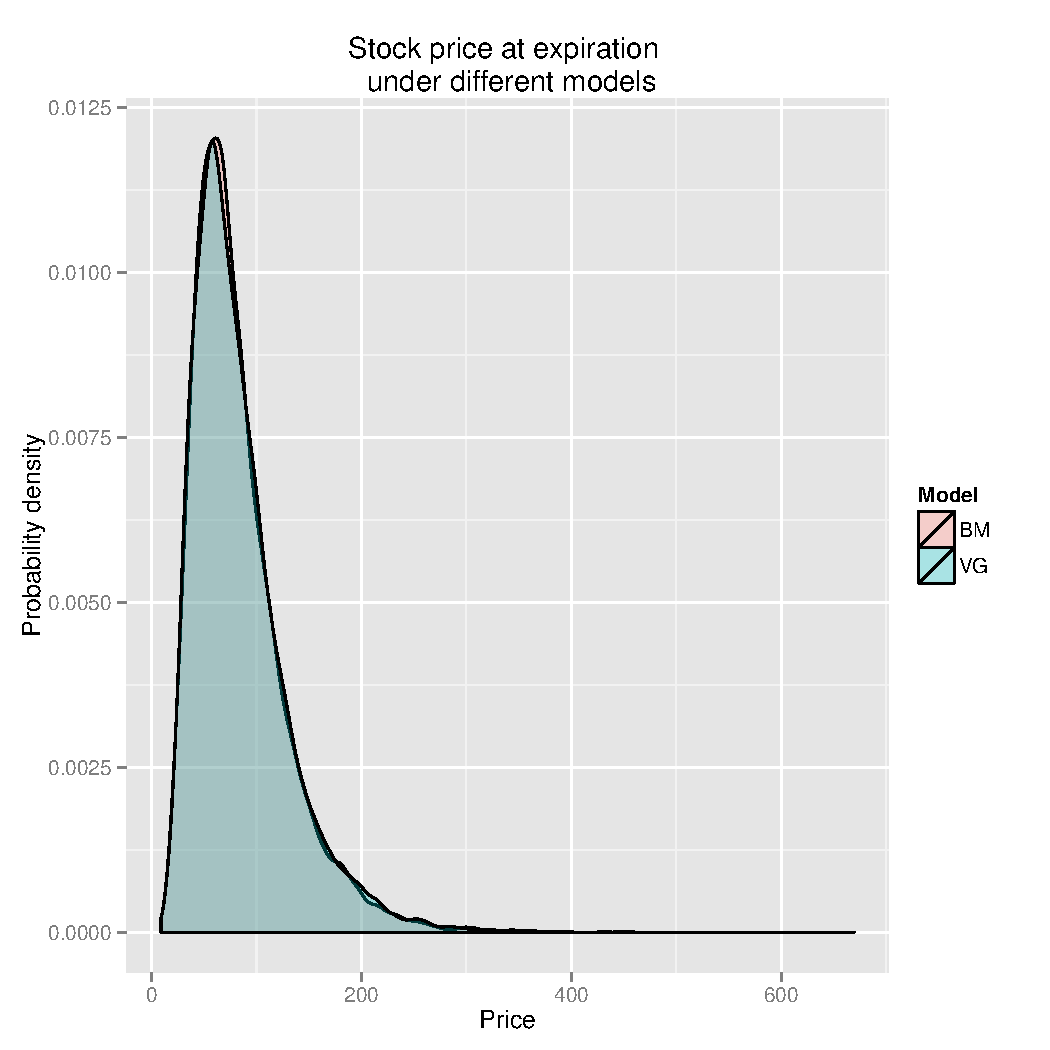
\includegraphics[width=1.0\textwidth]{fb}
\end{center}

\section{Conclusion}
We found that by using a model that allowed for fat tails, the price of call increases. By put-call-parity, which assumes nothing about the underlying measure, the price of a put increases too. The reason for this is because by writing an option, the seller creates an asymmetric exposure for him or herself. The small probability yet costly tail risk can only hurt him or her, and only help the contract holder. As evidenced by the anecdotes of Long-Term Capital Management and Nassim Taleb, these low probability events can make or break one's career in the derivatives markets.

\newpage

\bibliography{finalpaper}
\bibliographystyle{ieeetr}

\end{document}
